
\chapter{Model}\label{chap:model}

The purpose of this section is to present the techno-economic model used in this project. In the previous chapter, the mathematical framework of a techno-economic model was presented, and in this chapter, the physical interpretations of the equations making the model will be discussed. Furthermore, all the time-series and cost data used in the model will be presented. The model used in this project is heavily inspired by the work performed in \cite{PyPSA_euro_30_model}. 

\section{Topology}
The model used in this project is based on the work presented in \cite{PyPSA_euro_30_model}, where a model spanning the electricity grid of 30 European countries is formulated as a techno-economic linear optimization problem. Countries included in the model are the EU-28 countries not including Cyprus and Malta, instead of including Norway, Switzerland, Serbia, and Bosnia and Herzegovina.

The topology of the network presented in Figure \ref{fig:network_lay}, is such that each node represents a country and the links represent international HVDC or HVAC links. The links included are based on currently installed international transmission lines. 


\begin{figure}[h]\centering
	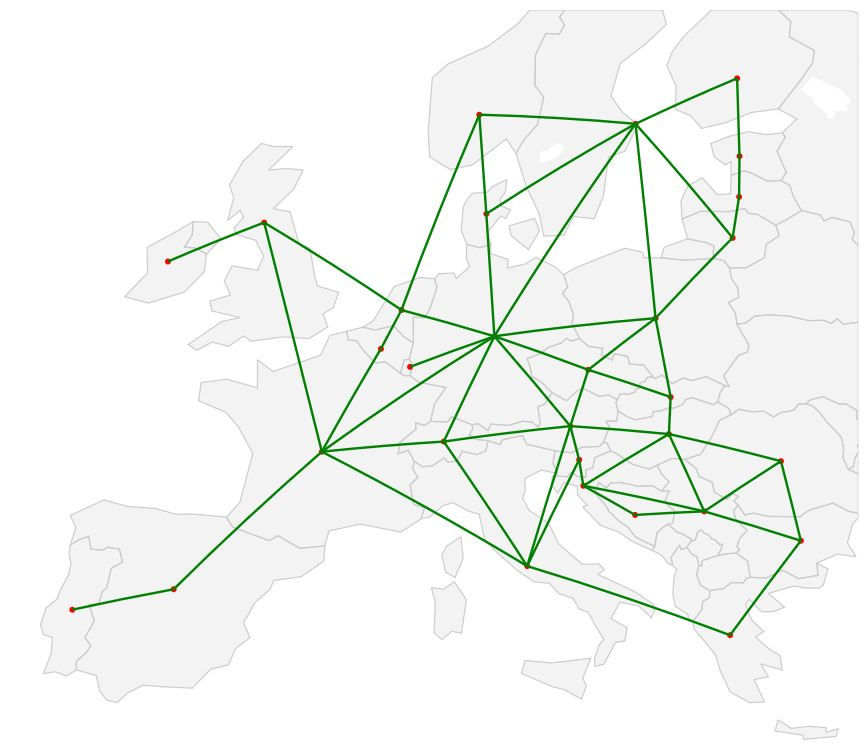
\includegraphics[width=0.75\textwidth]{./Images/network_layout}
	\caption{This figure shows the topology of the techno-economic model used in this project. Green lines represent transmission lines and red dots present the location of centroid of all countries included in the model.}
	\label{fig:network_lay}
\end{figure}


All model input parameters are based on 2011 values as this is the earliest year with all data available. The temporal resolution of the model is hourly, with all simulations spanning a full year. Technology costs are all valued in 2011 Euros. 

\section{Energy production}

Each node in the network, has energy-producing technologies available, with initial capacities being zero. The available energy-producing technologies used in this project: Onshore wind, offshore wind, solar PV and open-cycle gas turbines (OCGT). In the model, all technology capacities are expandable limited only be the geographical potential. 

The geographical potentials used are calculated following the work of  \cite{PyPSA_euro_30_model}. In the calculation of geographical potential, the potential available area suited for either onshore wind, offshore wind, and solar PV, must first be defined. These areas were found by allowing certain technologies to be installed only in areas with certain land-use types. Hereby restricting onshore wind farms from being installed in cities and solar PV plants from being installed in forests etc. The placement of offshore wind farms was restricted to areas with a water depth of less than 50m. Furthermore, all nature reserves were excluded from potential areas. As competing land use and likely public acceptance issues will occur, the found potential areas are set to bee only 20\% of the found area for onshore and offshore wind and only 1\% for solar PV. 
Assuming a maximum nominal installation density of 10 $MW/km^2$ for offshore and onshore wind power, and 145 $MW/km^2$ for solar PV \cite{PyPSA_euro_30_model}, it is possible to calculate the geographical potential for the three technologies all across Europe. 

The hourly energy production of all variable renewable energy sources is limited by the production potential given by the weather. Following \cite{PyPSA_euro_30_model}, the availability was calculated using historical weather data for 2011 from \cite{ClimateForecastSystem} with a spatial resolution of 40x40 km and hourly temporal resolution. The weather data is first converted to generation potentials for each 40x40 km cell using the REatlas software \cite{ANDRESEN20151074}, and then the national hourly means are found. The mean capacity factor for wind and solar power is presented in Figure \ref{fig:capacity_factor}.


\begin{figure}[h]\centerfloat
	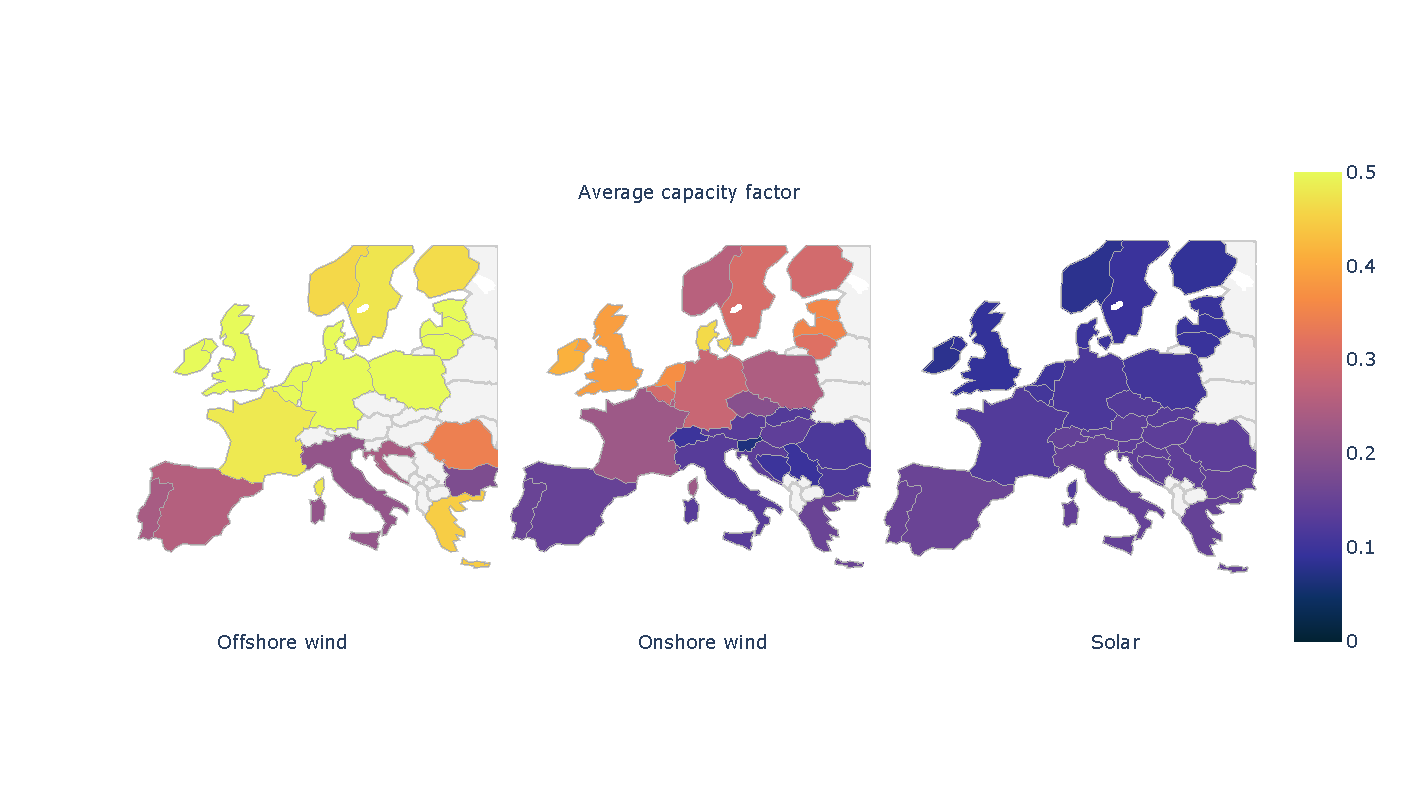
\includegraphics[width=1.3\textwidth]{./Images/wind_availability}
	\caption{The figure shows the average generation potential of wind turbines and solar PV plants, in the individual countries included in the model.  }
	\label{fig:capacity_factor}
\end{figure}



The dispatchable energy sources available in all countries are chosen to be open-cycle gas turbines (OCGT), as they have high flexibility and good load following capabilities, therefore making them suitable as a backup generator in a highly decarbonized scenario. They do however not necessarily produce realistic results when used in scenarios with low decarbonization, as other plant types such as conventional coal-powered combined heat and power perform better in these cases. The capacities and energy generation of the gas turbines are contrary to the variable renewable energy sources, not limited by geographical or generation potentials. They are, however, limited by the maximum allowable $\text{CO}_2$ emission. The $\text{CO}_2$ emission intensity of the open cycle gas turbine is 0.19 t/MW \cite{PyPSA_euro_30_model}. In this project, the $\text{CO}_2$ constraint will always be calculated as a percentage reduction in emission compared to a scenario run on the same model with the same parameters without any constraint on $\text{CO}_2$ emission. 

In countries located on the coast both onshore and offshore wind turbines are available. The capacity of these two types of wind power is however treated as one single variable in all simulations performed in this project. 

In all simulations, the capacities of all energy generators are initially set to be zero, with the capability to be expanded until geographical potentials or $\text{CO}_2$ constraints, limits further expansion. The cost of expanding capacities is calculated as annualized cost, given as the annualized investment cost plus fixed annual operations and maintenance cost. The annualized investment cost is calculated by multiplying the annuity factor (Equation \ref{eq:annuity}) by the investment cost. 

\begin{equation}\label{eq:annuity}
a = \frac{r}{1 - \frac{1}{(1+r)^n}}
\end{equation}

Where $r$ is the discount rate, and $n$ is the expected lifetime of the given technology. In this project a discount rate of 7\% \cite{PyPSA_euro_30_model} is used. The lifetime of the individual technologies are listed in Table \ref{tab:cost_data}. All cost data are based on the 2030 values presented in \cite{Schroder2013Current}.

\begin{table}[]
	\begin{tabular}{l|llll}
		Technology      & \makecell[c]{Investement \\ {[}€/MW{]}}    & \makecell[c]{Fixed O\&M \\ {[}€/kW/year{]}} & \makecell[c]{Marginal cost \\ {[}€/MWh{]}}    & \makecell[c]{lifetime \\ {[}years{]}} \\ \hline
		Onshore Wind    &       1182          &   35      &   0.015       &   25       \\
		Offshore Wind    &        2506        &    80        &    0.02        &    25        \\
		Solar PV           &       600            &   25      &   0.01        &   25       \\
		OCGT               &       400            &   15      &   58.4        &   30      \\
		Transmission    &   \makecell[l]{ 400 €/MW km \\ +150000€ pr line}  & 2\% & 0         &   40 
	\end{tabular}
	\caption{Generator parameters are based on the values from \cite{Schroder2013Current}, and transmission parameters are based on the work presented in \cite{HAGSPIEL2014654}.}
	\label{tab:cost_data}
\end{table}

\section{Energy demand}
The data for the hourly electricity demand found in the European Network of Transmission System Operators data portal is used as energy demand \cite{ENTSO-E}. The data has a resolution of one hour and is provided for all countries included in the model. In Figure \ref{fig:demand}, the summarized demand for the entire year for the individual countries is shown. A total of $3152$TWh of energy was consumed by the countries combined in 2011. 

\begin{figure}[h]\center 
	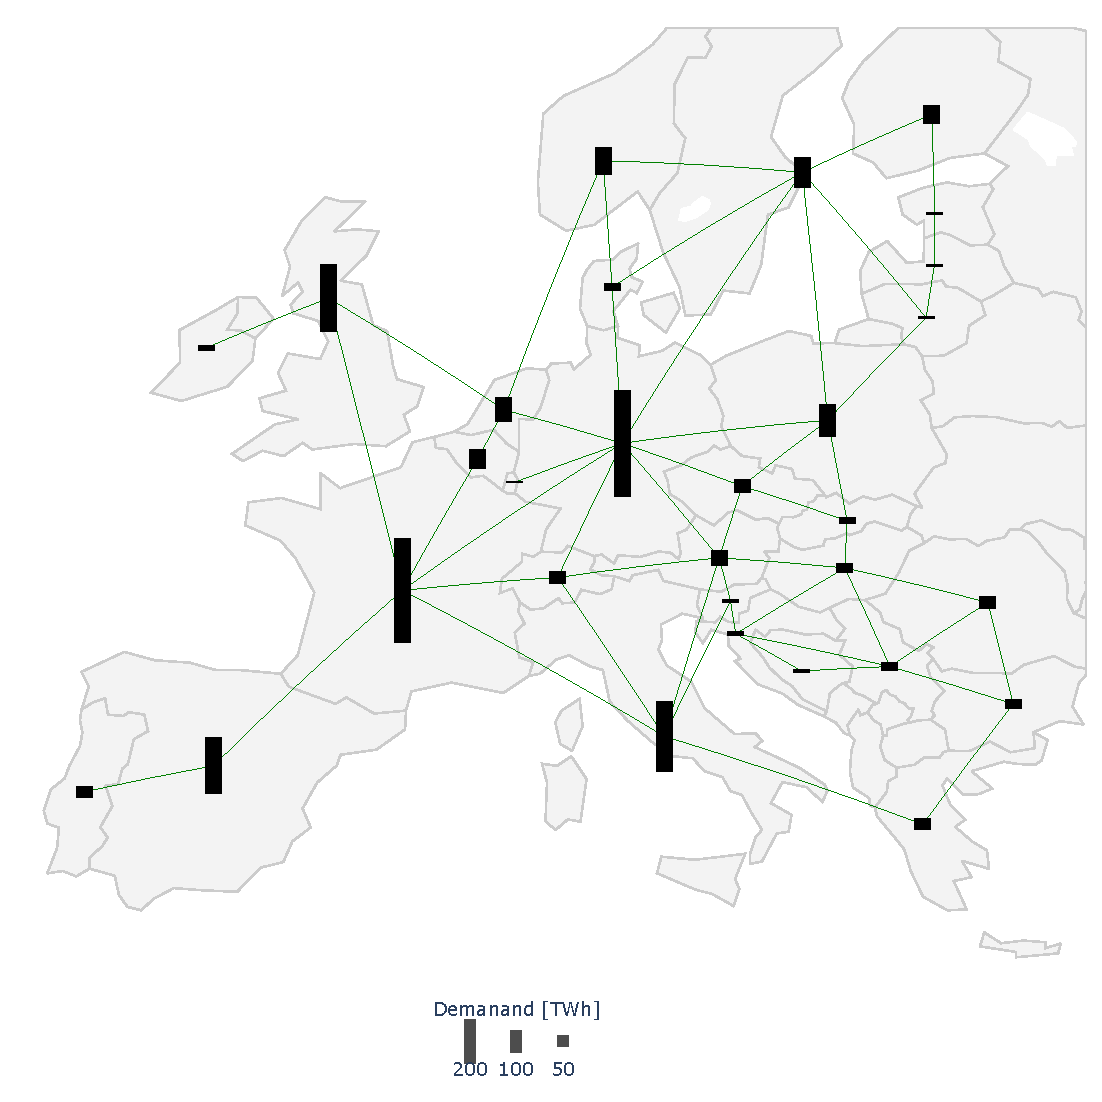
\includegraphics[width=.8\textwidth]{./Images/Demand}
	\caption{The figure shows the total electricity demand of the individual countries during an entire year. }
	\label{fig:demand}
\end{figure}

\section{Energy transmission}
In the model used in this project, all transmission lines are treated as transport models with a coupled source and sink, only constrained by energy conservation at each connecting node. Transmission loss is thereby not considered. This approximation is assumed to be acceptable as most international transmission lines already are, or probably will be in the near future, controllable point-to-point high voltage direct current (HVDC) lines. 

Line capacities initially start as zero, and can then be expanded if found feasible in the optimization, with no constraint on the maximum allowable capacity. The investment cost of line capacity is calculated as a cost pr MWkm plus an additional cost for a high voltage AC to DC converter pair. The price of a high voltage AC to DC converter pair is set to be 150000€ regardless of line capacity \cite{HAGSPIEL2014654}. 

The length of each line is set as the distance between the centroids of each connecting country plus an additional 25\%. The extra 25\% is added to the line length as competitive land use and public acceptance issues will prohibit lines from being placed in optimal positions. 

Furthermore, to satisfy n-1 security the price is adjusted with a factor of $1.5$, to account for the extra installed capacity needed, as shown in \cite{PyPSA_euro_30_model}. 

\begin{equation}
c_l = \left( L\cdot I_s \cdot 1.25+150000 \right) 1.5 \cdot 1.02 \cdot a
\end{equation}

%1.25 = 25\% extra length due to land use competition. 
%150000  Price of DC converter pair
%1.5 = n-1 security 
%1.02 = 2\% FOM (fixed operations and maintenance cost)
%a = annuity 



\section{Utilization of parallel programming and cluster computing}
As the MGA approach described in Section \ref{sec:Novel_MGA} requires a high number of similar optimizations to be performed only with slightly changed objective functions, it is possible to achieve a great performance boost, by utilizing parallel programming and cluster computing.

The model used in this project is implemented in the open-source tool PyPSA \cite{Pypsa}, build for the programming language Python. The individual optimizations of the model are done with the optimization tool Gurobi \cite{Gurobi}. The Gurobi solver is capable of using several computing cores to speed up the process of optimizing the model. Allowing Gurobi to use two cores, it is possible to find an optimal solution to the techno-economic model used in this project in approximately 20 minutes. As the MGA method presented in this project requires several optimizations of the problem, with a changing objective function, it is possible to reduce the computation time drastically by utilizing parallel programming. 

Using the Python framework  Multiprocessing \cite{Multiprocessing}, the MGA method presented in this project was implemented, capable of performing several optimizations at once. Using the PRIME compute cluster \cite{Prime}, it was possible to perform 16 parallel optimizations on the 32 core compute nodes, reducing the time needed per MGA study drastically. 
The Prime compute cluster \cite{Prime}, has 17 compute nodes with 24-36 cores available each operating at roughly 3 GHz, giving a total of 538 cores. Performing an MGA study requires anything in the range of 100-2000 optimizations of the model, each one requiring two cores for twenty minutes. Using a single compute node with 32 cores a single MGA study can be performed in a few hours up to two days, depending on the complexity of the problem. 

